\chapter{Transport Layer}

\begin{definitionbox}{test}
    text here
\end{definitionbox}

\section{The Transport Layer}
Provides connection (\textbf{TCP}) and connection-less (\textbf{UDP}) services to allow communication between \textbf{end-systems/hosts}.
\begin{itemize}
    \setlength\itemsep{0em}
    \item Connection decision is made at this level.
    \item Only runs on \textbf{end hosts}, not on \textbf{routers} or \textbf{switches}.
    \item Requires the lower layers in order to operate (Network, Data-link and Physical).
    \item Protocols in this layer work on the assumption that the lower levels are working, however must consider that \textbf{IP} is best effort, and gives no guarantees on data integrity or order of delivery for packets.
\end{itemize}

Other layer-4/Transport Layer protocols include:
\begin{center}
    \begin{tabular}{l p{0.8\textwidth}}
        \textbf{QUIC}     & A \textbf{UDP} based transport layer designed by google employees to replace \textbf{TCP} using multiple multiplexed connections using \textbf{UDP}, focused on improving \textbf{HTTP} performance. The \href{https://en.wikipedia.org/wiki/QUIC}{wikipedia article} goes into more detail.  \\
        \textbf{UDP-Lite} & A \textbf{UDP} like connectionless protocol that allows potentially damaged data payloads to be propagated to the application layer, and hence allows the application layer to discern data integrity and act accordingly (\href{https://en.wikipedia.org/wiki/UDP-Lite}{Wikipedia article}). \\
        \textbf{DCCP}     & The \textbf{Datagram Congestion Control Protocol} is a message-oriented protocol that uses reliable connection setup, close and has explicit congestion notification (\href{https://en.wikipedia.org/wiki/Datagram_Congestion_Control_Protocol}{Wikipedia article}).                          \\
        \textbf{SCTP}     & The \textbf{Stream Control Transmission Protocol} is a message-oriented protocol based on \textbf{UDP} (\href{https://en.wikipedia.org/wiki/Stream_Control_Transmission_Protocol}{Wikipedia article}).                                                                                        \\
        \textbf{RSVP}     & The \textbf{Resource Reservation Protocol} is used to reserve network resources to ensure quality of service (\href{https://en.wikipedia.org/wiki/Resource_Reservation_Protocol}{Wikipedia article}).                                                                                         \\
    \end{tabular}
\end{center}

\section{Terminology}
\begin{center}
    \begin{tabular}{l l l}
        \textbf{Layer}   & \textbf{No} & \textbf{Data Name}                                       \\
        \hline
        Application      & 5           & Data                                                     \\
        Transport        & 4           & TCP Segments (created by segmentation) or UDP Datagrams  \\
        Network/Internet & 3           & IP Datagrams (a.k.a. packets) (created by fragmentation) \\
        Data Link        & 2           & Frames                                                   \\
        Physical         & 1           & Bits                                                     \\
    \end{tabular}
\end{center}

\section{Port Numbers}
\begin{definitionbox}{Ports}
    Used to connect applications together/ separate different application's connections.
    \\
    \\ The transport layer uses port numbers to differentiate between many different network communications. Each application on a host uses a unique port number.
    \\
    \\ Port numbers are cross-platform, meaning on many different devices, computer architectures and OSes they are the same for the same types of applications (e.g HTTP, IMAP).
    \begin{center}
        \begin{tabular}{c c c l}
            \multicolumn{3}{c}{\textbf{Ports}} & \textbf{Use}                                                                                                         \\
            \hline
            $0$                                & $\to$        & $1023$  & (well known/reserved for certain protocols, e.g HTTP $\to 80$, SMTP $\to 25$, SSH $\to 22$) \\
            $1024$                             & $\to$        & $49151$ & (for any user application to use or register)                                               \\
            $49152$                            & $\to$        & $65535$ & (dynamic/ephemeral/private) and are used by clients temporarily)                            \\
        \end{tabular}
    \end{center}
\end{definitionbox}

\section{TCP}
\begin{definitionbox}{Transmission Control Protocol (TCP)}
    A connection-oriented transport layer protocol.
    \begin{itemize}
        \setlength\itemsep{0em}
        \item Data is split into \textbf{segments}.
        \item Reliable data transfer (integrity of data and (possibly) ordered delivery)
        \item Not secure (other mechanisms need to be used to ensure security)
        \item Can offer stream connections (ordered delivery, only accept segments in order, e.g received $4$, waiting for $5$, but received $6,7$, ignore $6$ and $7$ until $5$ is received.)
        \item Congestion Control (avoids destructive congestion on the network)
        \item Requires A handshake to start the connection.
        \item \textbf{Full-Duplex} so both sides can send and receive at the same time.
    \end{itemize}
\end{definitionbox}

To identify a socket connection we use the \textbf{IP Address}, port number and protocol (\textbf{TCP}/\textbf{UDP}).
\begin{center}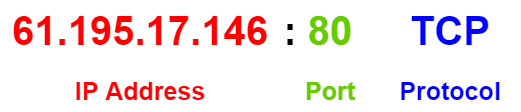
\includegraphics[width=0.7\textwidth]{transport_layer/images/socket id.png}\end{center}

\begin{definitionbox}{Berkely Socket Interface}
    An interface adopted by all \textbf{UNIX} systems and windows.
    \begin{center}
        \begin{tabular}{l p{0.7\textwidth}}
            \textbf{1. }\fun{SOCKET}  & Create a new communication endpoint.                                                                                                                        \\
            \textbf{2. }\fun{BIND}    & Attach a local address to the socket. The client and server both bind a transport level address and name to the locally created socket.                     \\
            \textbf{3. }\fun{LISTEN}  & Prepare for / Announce ability to accept, $n$ connections. The kernel now waits for connections from clients.                                               \\
            \textbf{4. }\fun{ACCEPT}  & Block until some remove client wants to establish a connection, hence the server can now wait, receive a request and choose to accept or deny a connection. \\
            \textbf{5. }\fun{CONNECT} & Attempt to establish a connection. When a client connects it must provide the full transport-level address to locate the socket.                            \\
            \textbf{6. }\fun{SEND}    & Send data over the connection.                                                                                                                              \\
            \textbf{7. }\fun{RECEIVE} & Receive data over a connection.                                                                                                                             \\
            \textbf{8. }\fun{CLOSE}   & Release the connection, communication ends when the socket is closed.                                                                                       \\
        \end{tabular}
    \end{center}
    A connection-oriented example:
    \begin{center}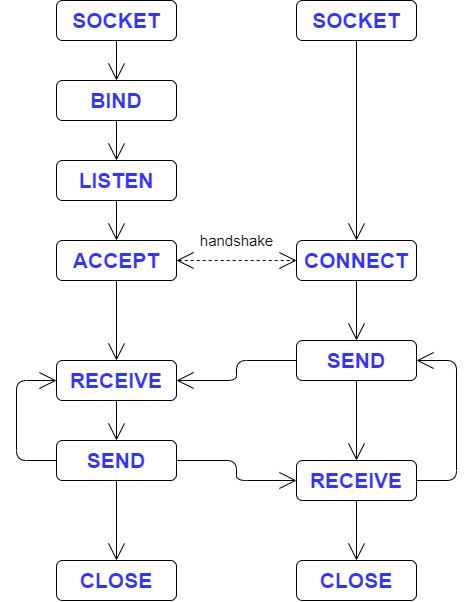
\includegraphics[width=0.6\textwidth]{transport_layer/images/berkely interface.png}\end{center}
    In a connection-less scenario, \fun{LISTEN}, \fun{ACCEPT} and \fun{CONNECT} are not required.
\end{definitionbox}
\begin{examplebox}{Simple Java Web Client}
    \center\begin{minipage}[t]{0.9\textwidth}
        \inputminted{Java}{transport_layer/code/exampleTCPClient.java}
    \end{minipage}
\end{examplebox}
\begin{examplebox}{Simple Java Web Server}
    \begin{center}
        \begin{minipage}[t]{0.9\textwidth}
            \inputminted{Java}{transport_layer/code/exampleTCPServer.java}
        \end{minipage}
    \end{center}
    To handle many clients, a thread must be created per client, rather than the basic forever loop as above.
\end{examplebox}

\subsection{Segments}
\begin{definitionbox}{TCP Segment}
    A wrapper for \textbf{TCP} data, transmitted within the Network Layer protocol (e.g \textbf{IPv4} or \textbf{IPv6})
\end{definitionbox}
\begin{definitionbox}{Maximum Segment Size (MSS)}
    The maximum amount of application data transmitted in a single segment (header size is not included).
    \\
    \\ Usually related to the \textbf{MTU} of the connection to avoid network level fragmentation (splitting segments in the network layer into multiple packets).
\end{definitionbox}
\begin{definitionbox}{Maximum Transmission Unit (MTU)}
    The largest link layer frame available to the sender. Consider it as the largest unit of data that can be transmitted through all links to the receiver without requiring it to be split.
    \\
    \\ \textbf{Path MTU Discovery} determines the largest frame that can be sent on all links from the sender to receiver.
\end{definitionbox}

\subsection{TCP Header}
From the \href{https://nmap.org/book/}{NMap book}:
\begin{center}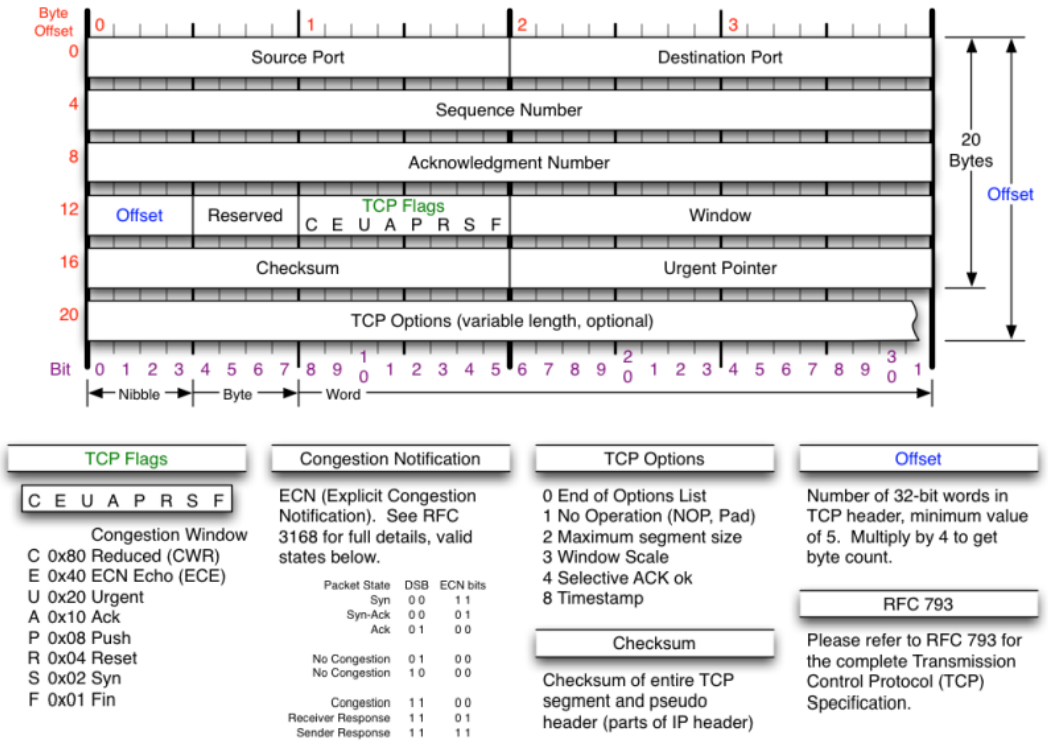
\includegraphics[width=0.7\textwidth]{transport_layer/images/nmap book.png}\end{center}
Points of note:
\begin{itemize}
    \setlength\itemsep{0em}
    \item Source and destination ports are $16$ bit identifiers.
    \item Sequence number and Acknowledgement Number ($32$ bits) is used for reliable data transfer (identifies a segment, so any segments missing in the sequence can be detected)
    \item Receive window ($16$ bits), the amount of data that can be sent before an acknowledgement is received (if the receiver cannot process data as fast as it arrives, it will ask to reduce the TCP window), more \href{https://accedian.com/blog/tcp-receive-window-everything-need-know/}{here}.
    \item Header length determines the size of the \textbf{TCP} header in $32$ bit words.
    \item The optional/variable length field is used to negotiate protocol parameters such as window scale, or \textbf{maximum segment size}.
\end{itemize}
There are several header Fields:
\begin{center}
    \begin{tabular}{l l p{0.7\textwidth}}
        \textbf{Field} & \textbf{Bits} & \textbf{Description}                                                                                                             \\
        \hline
        \const{URG}    & $1$           & Signals the data as urgent, location of urgent data marked by urgent data pointer field. Note that some software will ignore it. \\
        \const{ACK}    & $1$           & Signals that the acknowledgement number is a valid acknowledgement.                                                              \\
        \const{PSH}    & $1$           & Push flag, asks the receiver to push data to the application immediately.                                                        \\
        \const{RST}    & $1$           & Resets the connection, often used to shutdown a connection when some unexpected error occurs.                                    \\
        \const{SYN}    & $1$           & Synchronisation flag, used as part of the handshake.                                                                             \\
        \const{FIN}    & $1$           & Signals connection to finish/shutdown.                                                                                           \\
        Checksum       & $16$          & Used for error detection.                                                                                                        \\
    \end{tabular}
\end{center}
\begin{definitionbox}{Sequence Number}
    Each byte in the data stream has a sequence number (byte, \textbf{not} segment).
    \\
    \\ The sequence number in a \textbf{TCP segment} indicates the position of the first byte carried by that segment.
    \begin{center}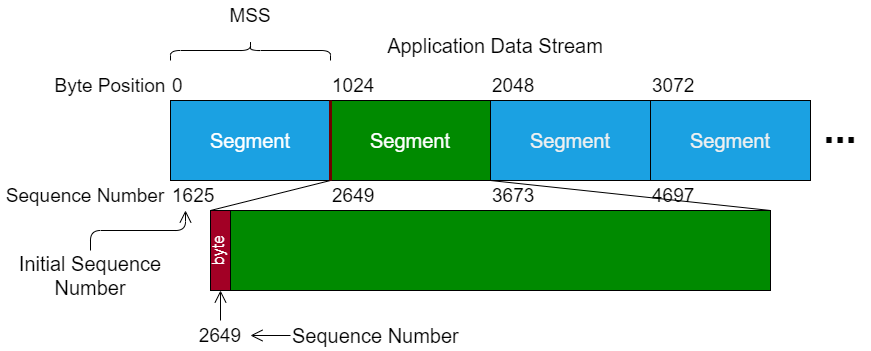
\includegraphics[width=0.8\textwidth]{transport_layer/images/sequence number.png}\end{center}
    When the \textbf{TCP} connection is setup, a random \textbf{Initial Sequence Number} is decided upon to avoid any leftover segments being received by mistake.
    \\
    \\ Hence when creating a new connections, even with the same data the sequence numbers will be different.
\end{definitionbox}
\begin{definitionbox}{Acknowledgement Number}
    An \textbf{acknowledgedment number} represents the end of the data received, or the first sequence number  of the data waiting to be received.
    \begin{itemize}
        \setlength\itemsep{0em}
        \item TCP acknowledgements can be cumulative (recieve segments $1,2,3$, ackenowledge (wait for) $4$).
        \item Typically acknowledge every other packet.
    \end{itemize}
    \begin{center}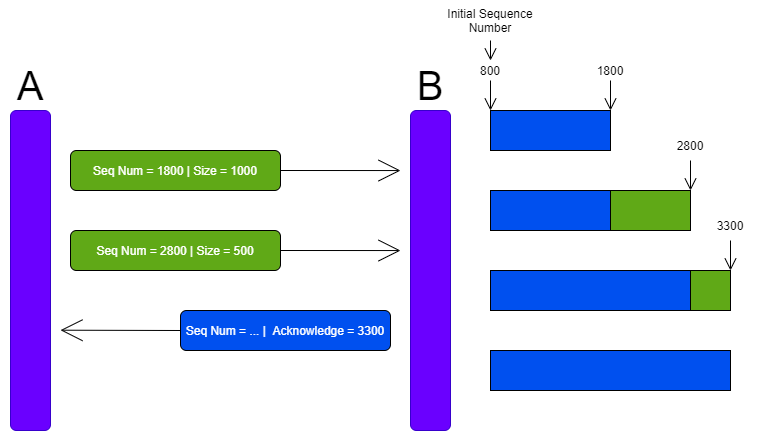
\includegraphics[width=\textwidth]{transport_layer/images/tcp acknowledgement.png}\end{center}
    \begin{itemize}
        \setlength\itemsep{0em}
        \item As \textbf{TCP} is full duplex, multiple streams/sequences can be received, and acknowledged at the same time.
    \end{itemize}
\end{definitionbox}

\subsection{3-Way Handshake}
\begin{enumerate}
    \setlength\itemsep{0em}
    \item Client sends a \textbf{TCP segment} with the \const{SYN} flag set to \const{true}, and the \textbf{initial sequence number}.
    \item Server responds with another \const{SYN} \textbf{TCP segment} which also has \const{ACK} as \const{true} and the first unseen client Sequence number.
    \item Client responds with an \const{ACK} with first unseen server \textbf{sequence number}, and a new \textbf{sequence number}.
\end{enumerate}
\begin{center}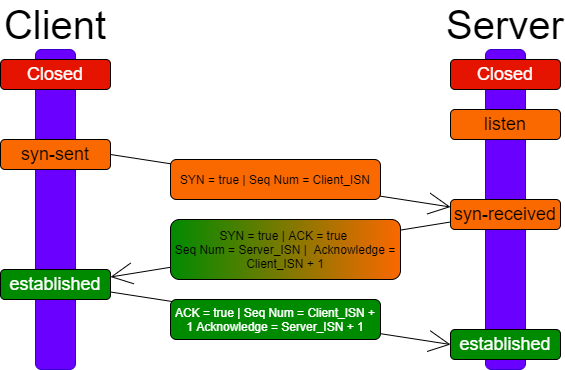
\includegraphics[width=0.6\textwidth]{transport_layer/images/3 way handshake.png}\end{center}
Connection termination is similar, but uses \const{FIN}.

\section{UDP}

\begin{definitionbox}{User Datagram Protocol (UDP)}
    A connection-less transport layer protocol.
    \begin{itemize}
        \setlength\itemsep{0em}
        \item Data is split into \textbf{datagrams} (think like telegrams).
        \item \textbf{Datagrams} cannot be larger than $65,507$ bytes ($20B$ IP Header $+ 8B$ UDP Header + $65,507B = 65,535B$ which is the maximum IP packet size).
        \item In practice smaller $500B \to 1KB$ datagrams are used to increase the proportion of packets that are intact (any small error only effects a small datagram, does not invalidate a large datagram).
        \item Application identification is provided (multiplexing/demultiplexing).
        \item Integrity of data is checked by a \href{https://en.wikipedia.org/wiki/Cyclic_redundancy_check}{\textbf{CRC}}-type checksum.
    \end{itemize}
    \textbf{UDP} is very simple:
    \begin{itemize}
        \setlength\itemsep{0em}
        \item no flow Control
        \item no error Control
        \item no retransmissions
    \end{itemize}
    Why use \textbf{UDP}?
    \begin{itemize}
        \setlength\itemsep{0em}
        \item Finer level of application layer control over when and what data is sent (e.g real-time such as skype).
        \item No connection needs to be established (faster than TCP).
        \item No connection state needs to be stored.
        \item Very small packet overhead (only a small bit of the packet is not payload).
    \end{itemize}
    It is also very useful in \textbf{client-server} interactions.
    \\
    \\ A client can send a short message to a server, and get a quick response, on failure can time out or try again. The resulting code is simple and fewer messages are needed (no connection setup/teardown).
\end{definitionbox}
\subsection{UDP Header}
\begin{center}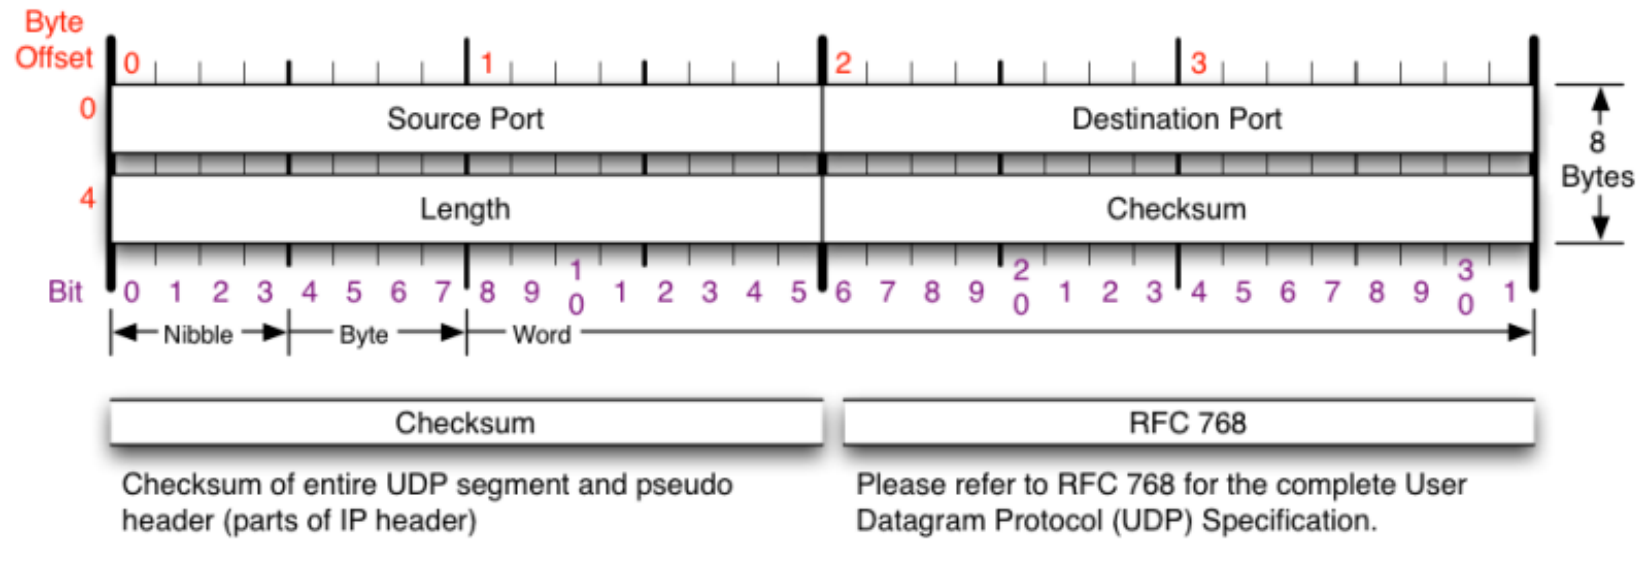
\includegraphics[width=0.9\textwidth]{transport_layer/images/nmap book udp.png}\end{center}

\begin{examplebox}{Simple Java Web Client}
    \center\begin{minipage}[t]{0.9\textwidth}
        \inputminted{Java}{transport_layer/code/exampleUDPClient.java}
    \end{minipage}
\end{examplebox}
\begin{examplebox}{Simple Java Web Server}
    \center\begin{minipage}[t]{0.9\textwidth}
        \inputminted{Java}{transport_layer/code/exampleUDPServer.java}
    \end{minipage}
\end{examplebox}

\section{TCP vs UDP}
\begin{itemize}
    \bullpara{(UDP) - A PvP Game sending short bursts of data to players}{
        \\ Data transmission is time critical, if a message is lost, we can simply recover our own way (e.g list of messages, retry).
        \\
        \\ We get to control the implementation. While we may mimic TCP in some error recovery, we can decide what features we want and don't for the best experience.
    }
    \bullpara{(TCP) - An online card game}{
        \\ Speed is not a concern, \textbf{TCP} is just fine.
    }
    \bullpara{(TCP) - Movie player application}{
    \\ We want it to be fast, however we do not want to drop frames.
    \begin{itemize}
        \setlength\itemsep{0em}
        \item Pre-Buffer the video, and constantly use connection to get next few seconds as the movie plays.
        \item TCP manages errors to reduce dropped frames.
              }
    \end{itemize}
\end{itemize}

\section{Data Transfer}
\begin{definitionbox}{(FSM) Finite State Machine}
    A mathematical abstraction used among other uses, to describe network protocols.
    \begin{center}
        \begin{tabular}{l l l}
            FSM & Finite State Machine                      \\
            FSA & Finite State Automata                     \\
            DFA & Deterministic finite-state automaton      \\
            NFA & None-deterministic finite state automaton \\
        \end{tabular}
    \end{center}
\end{definitionbox}
We can describe transitions between states for a protocol by the event and action.
\begin{examplebox}{Among Us Basic Group Meeting}
    \begin{center}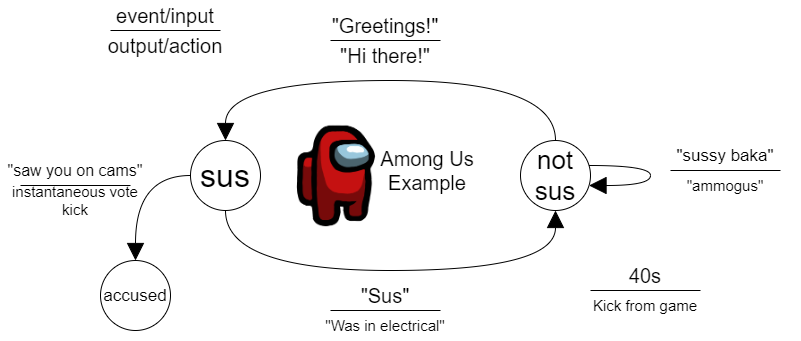
\includegraphics[width=0.7\textwidth]{transport_layer/images/example fsm.png}\end{center}
\end{examplebox}
\subsection{TCP FSM}
\begin{center}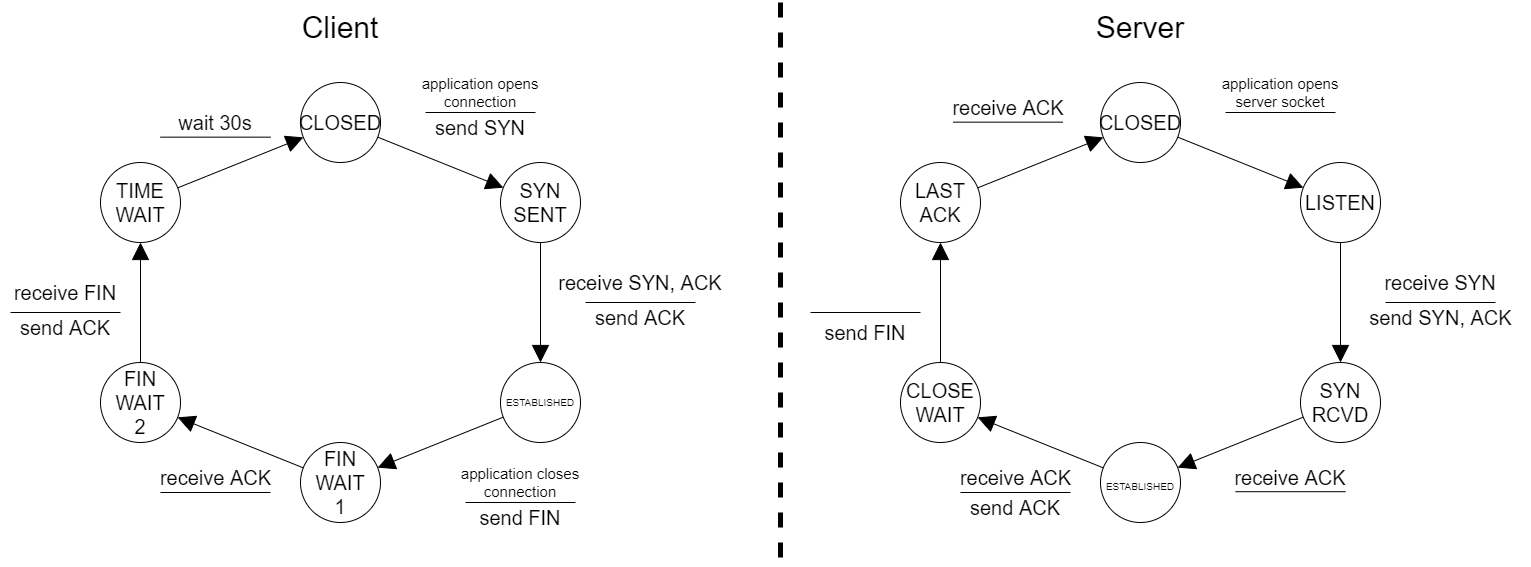
\includegraphics[width=\textwidth]{transport_layer/images/tcp fsm.png}\end{center}
\begin{sidenotebox}{View TCP states on your device}
    On windows can use \fun{netstat -a} \href{https://docs.microsoft.com/en-us/sysinternals/downloads/tcpview}{tcpview} or \href{https://www.nirsoft.net/utils/cports.html}{currPorts}.
    \\
    \\ On linux there is \href{https://htop.dev/}{htop} and \href{http://iptraf.seul.org/}{iptraf}.
\end{sidenotebox}

\subsection{Data Transfer FSM}
\textbf{TCP} provides mechanisms to ensure reliability in data transfer. While \textbf{IP} in the \textbf{Network Layer} is a best-effort protocol and is unreliable, by going through \textbf{TCP} we can create a reliable connection.
\\
\\ we can generalise this as:
\begin{center}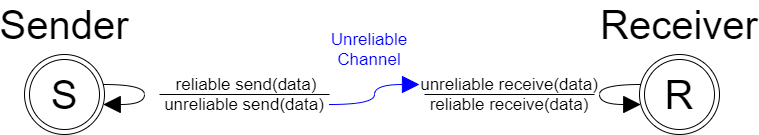
\includegraphics[width=\textwidth]{transport_layer/images/data transfer fsm.png}\end{center}

\subsection{Error Detection}
Bits may be flipped in transmission (due to noise/interference and imperfect physical hardware).
\begin{center}
    \begin{tabular}{l p{0.8\textwidth}}
        \textbf{Error Detection}   & Receiver must be able to check if packet is corrupted.              \\
        \textbf{Receiver Feedback} & Receiver must be able to tell sender the packet sent was corrupted. \\
    \end{tabular}
\end{center}

\begin{definitionbox}{Parity Bit}
    A very simple type of error dectection code, where a single bit is set based on the parity of the rest of the packet. Typically this is the \fun{XOR} of all the bits.
    \[\begin{matrix}
            1001 & \to & 1001 \ 0 \\
            1101 & \to & 1101 \ 1 \\
        \end{matrix}\]
\end{definitionbox}

\subsubsection{Stop and Wait with Error detection}
We can express the data transfer \textbf{FSM} to include error detection. In this setup the protocol is synchronous, meaning for each segment the sender must receive back an acknowledgement before the next segment is sent.
\begin{center}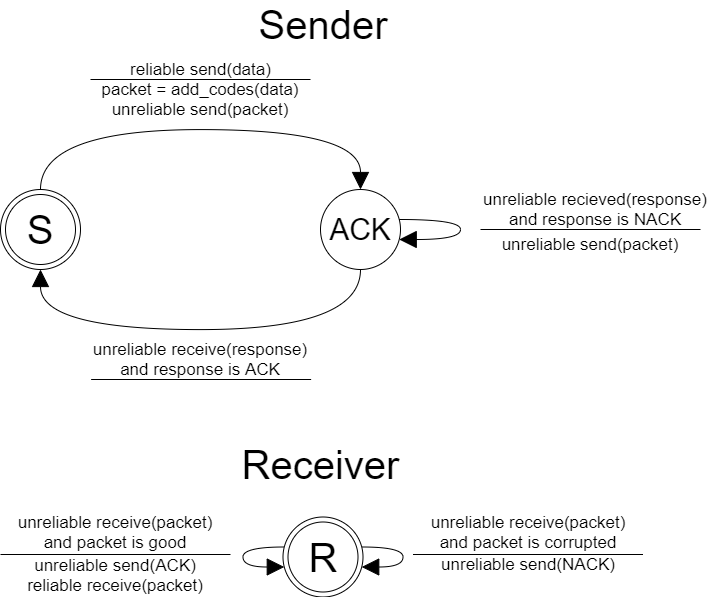
\includegraphics[width=0.8\textwidth]{transport_layer/images/data transfer error detection.png}\end{center}
The main issue with this approach, is that \const{ACK}s and \const{NACK}s can also get corrupted. If we use the same scheme to reliably transfer the \const{ACK}s and \const{NACK}s we end up with potentially no termination (sender and receiver stuck in a loop of replying with \const{NACK}s at each other, that the other does not receive uncorrupted on a noisy channel).

\subsubsection{Assume NACK and retransmit}
We can add a sequence number to each packet, so that packets can be retransmitted, and the receiver knows which packets are retransmissions.
\\
\\ If we use \textbf{stop and wait} we only need 1 bit for the sequence number, as $0$ is original, $1$ is retransmission.

\subsubsection{Use Sequence Numbers instead of NACKs}
We can instead use sequence numbers. If the packet is not acknowledged then an \const{ACK} is not sent. \const{ACK} is sent for the last good packet, hence the receiver can use a lack of \const{ACK}s to determine that it must retransmit some data.
\\
\\ Note that with TCP the \const{ACK} contains the start of the packet to be sent (or resent) next/ the end  byte sequence number of the data received.

\subsubsection{Out of Order Sequence Numbers}
Rather than use stop and wait, a sender may send many packets.
\begin{itemize}
    \setlength\itemsep{0em}
    \bullpara{Delayed \const{ACK}}{
        \\ The receiver only accepts in order, so ignores any packets sent out of order. After receiving a packet in order, it waits some time (e.g $500ms$) before sending the \const{ACK}, allowing for more in order-packets to be received in this time (resetting the wait).
        \begin{center}
            \begin{tabular}{l l}
                1. & Received $0$, start wait                                                            \\
                2. & Wait interrupted, received $1$, start wait again                                    \\
                3. & Wait interrupted, received $2$, start wait again                                    \\
                4. & Received $7$, ignored                                                               \\
                5. & Received $6$, ignored                                                               \\
                6. & Wait from (3.) over, send \const{ACK} (have recieved up to $2$, please send me $3$) \\
                   & \dots                                                                               \\
            \end{tabular}
        \end{center}
    }
    \bullpara{Cumulative \const{ACK}}{
        \\ Received an in-order segment with the expected number, waiting on the next segment.
        \\
        \\ Immediately send a cumulative \const{ACK}.
    }
    \bullpara{Duplicate \const{ACK}}{
        \\ Send an \const{ACK} for the next segment. Then an out-of-order segment arrived with a higher than expected sequence number, there is a gap.
        \\
        \\ Immediately send another (duplicate) \const{ACK}.
    }
    \bullpara{Immediate \const{ACK}}{
        \\ A segment received partially or completely fills a gap in the received data.
        \\
        \\ Immediately send an \const{ACK} for the lower end of the gap (to fill).
    }
\end{itemize}

\subsubsection{Timeouts}
We can set a timeout for receiving \const{ACK}s. When the sender does not receive an acknowledgment within the time, it assumes the packet was not received and can try again (retransmit).
\begin{itemize}
    \setlength\itemsep{0em}
    \item If the timeout is too long, when packets are lost retransmission will have to wait a long time and hence slow down the connection.
    \item If the timeout is too short, packets may be needlessly retransmitted.
\end{itemize}
\subsection{TCP \& Checksums}
Used by \textbf{TCP}. A checksum is calculated from the payload data.
\begin{itemize}
    \setlength\itemsep{0em}
    \item When received, if the checksum does not match the recalculated checksum, then corruption has occurred.
    \item Retransmission allows for error recovery.
    \item \const{ACK}s and \const{NACK}s are also protected by error detection code.
    \item Corrupted \const{ACK}s are used as \const{NACK}s
    \item Sequence numbers allow the receiver to ignore duplicate segments.
\end{itemize}

\section{Network Simulation}
We can use network simulation to check, test and optimise parameters for protocols and network designs.
\begin{itemize}
    \setlength\itemsep{0em}
    \bullpara{Cisco Packet Tracer}{
        \\ \href{https://www.netacad.com/courses/packet-tracer}{Packet tracer} is a lightweight network simulator with a user friendly GUI.
    }
    \bullpara{GNS3 Network Emulator}{
        \\ \href{https://www.gns3.com/}{GNS3} is network simulation tool available for free.
    }
    \bullpara{Opnet Modeler}{
        \\ \href{https://opnetprojects.com/opnet-network-simulator/}{Opnet} (now riverbed) modeller is a commercial (paid for) network simulation tool.
    }
\end{itemize}

\section{Detecting Congestion}
\begin{definitionbox}{Congestion}
    So far we have roughly described the \textbf{TCP Reno} protocol. However there are many other variants to deal with congestion control.
    \\
    \\ Routers have a limit to how many packets they can route. Packets are held in a queue.
    \\
    \\ If too many packets are sent to one of the routers between a sender and reciever, its queue will overflow, resulting in some segments being dropped.
    \\
    \\ Hence the server assumes the network is congested when it detects segment loss from:
    \begin{itemize}
        \setlength\itemsep{0em}
        \item timeouts (no \const{ACK} received)
        \item multiple \const{ACK}s (or equivalent acknowledgements) can be considered a \const{NACK}
    \end{itemize}
\end{definitionbox}

There are many different congestion control algorithms:
\\ \begin{minipage}{0.45\textwidth}
    \begin{center}
        \begin{tabular}{l l}
            \textbf{Algorithm}                                 & \textbf{Affects}         \\
            \hline
            TFRC                                               & Sender, Receiver         \\
            RED                                                & Router                   \\
            CLAMP                                              & Router, Receiver         \\
            XCP                                                & Sender, Router, Receiver \\
            VCP                                                & Sender, Router, Receiver \\
            MaxNet                                             & Sender, Router, Receiver \\
            JetMax                                             & Sender, Router, Receiver \\
            ECN                                                & Sender, Router, Receiver \\
            Vegas                                              & Sender                   \\
            High Speed                                         & Sender                   \\
            BIC                                                & Sender                   \\
            CUBIC                                              & Sender                   \\
            H-TCP                                              & Sender                   \\
            FAST                                               & Sender                   \\
            Compound TCP                                       & Sender                   \\
            Westwood                                           & Sender                   \\
            Jersey                                             & Sender                   \\
            \href{https://research.google/pubs/pub45646/}{BBR} & Sender                   \\
        \end{tabular}
    \end{center}
\end{minipage}
\hfill
\begin{minipage}{0.55\textwidth}
    \begin{itemize}
        \bullpara{Linux}{
            \\ Usually CUBIC, but can be found at \lstinline{/proc/sys/net/ipv4/tcp_congestion_control}.
        }
        \bullpara{Windows}{
            \\ Can be found at \lstinline{netsh interface tcp>sh gl}, if nothing then it is using the windows default.
        }
        \bullpara{Custom}{
            \\It is possible to force any socket to use any variant
        }
        \bullpara{Characteristics}{
            \\ Most have variable characteristics combined. For example:
            \begin{center}
                \begin{tabular}{l l}
                    Tahoe & Slow start, AIMD, Fast Retransmit \\
                    Reno  & Fast Recovery                     \\
                    Vegas & Congestion Avoidance              \\
                \end{tabular}
            \end{center}
        }
    \end{itemize}
\end{minipage}
\begin{definitionbox}{TCP Vegas}
    A popular \textbf{TCP} implementation.
    \begin{itemize}
        \setlength\itemsep{0em}
        \item Attempts to detect congestion before losses occur.
        \item Predicts packet loss using \textbf{RTT} (round trip time)
        \item Larger \textbf{RTT} $\Rightarrow$ greater congestion
    \end{itemize}
\end{definitionbox}
\begin{definitionbox}{TCP CUBIC}
    Used by linux as the standard.
    \\
    \\ In order to avoid advantaging smaller \textbf{RTT}s (as can happen with \textbf{TCP Reno}), grows \textbf{window} as a function of time rather than \textbf{RTT}
\end{definitionbox}

\begin{definitionbox}{Congestion Window}
    \begin{center}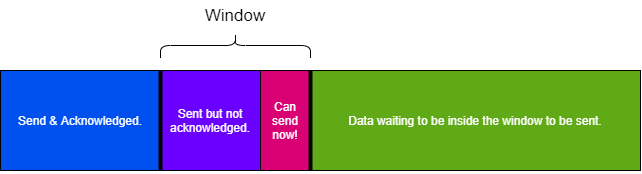
\includegraphics[width=0.7\textwidth]{transport_layer/images/TCP congestion window.png}\end{center}
    The \textbf{congestion window} is the number of bytes that can be sent before blocking to wait for acknowledgements.
    \\
    \\ Both the sender and receiver can define the window size, the size used is the minimum of both.
    \[W = min(\text{Congestion Window}, \text{Receiver Window})\]
    Hence with a given $RTT$ and window size $W$:
    \[\text{maximum rate } \ \lambda \approx \cfrac{W}{RTT}\]
\end{definitionbox}

\subsection{Congestion Methods}
\begin{definitionbox}{Slow Start}
    \begin{center}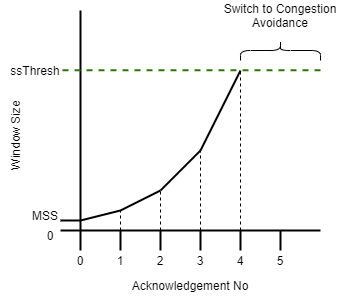
\includegraphics[width=0.6\textwidth]{transport_layer/images/slow start.png}\end{center}
    \begin{enumerate}
        \setlength\itemsep{0em}
        \item Set initial window size to \textbf{MSS} (maximum segment size) (quite small for high-speed networks).
        \item For every good acknowledgement, increase the window size by the size of data acknowledged (meaning window size is roughly doubled every \textbf{RTT}).
        \item Continue this exponential increase until window size reaches the \textbf{ssthresh} (segment size threshold).
        \item The use \textbf{Congestion Avoidance}.
    \end{enumerate}
\end{definitionbox}
\begin{definitionbox}{Congestion Avoidance}
    \begin{center}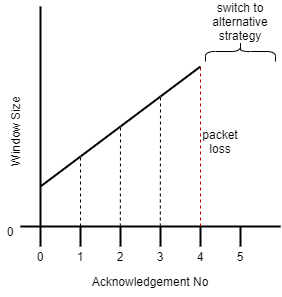
\includegraphics[width=0.6\textwidth]{transport_layer/images/congestion avoidance.png}\end{center}
    The window size is increased roughly linearly ($\approx 1 \ MSS$ per $RTT$).
    \\
    \\ For each good acknowledgement:
    \[W = W + \cfrac{MSS^2}{W}\]
    When congestion is detected (packet loss) switch to a different strategy.
\end{definitionbox}
\begin{definitionbox}{(AIMD) Additive Increase / Multiplicative Decrease}
    \begin{center}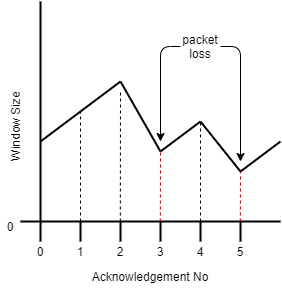
\includegraphics[width=0.5\textwidth]{transport_layer/images/AIMD.png}\end{center}
    \begin{itemize}
        \setlength\itemsep{0em}
        \item For every good acknoledgement: $W = W + \cfrac{MSS^2}{W}$
        \item For every packet loss event: $W = \cfrac{W}{2}$
    \end{itemize}
\end{definitionbox}
\begin{definitionbox}{timeout}
    We need to detect packet loss, when no \const{ACK} is send back.
    \begin{itemize}
        \setlength\itemsep{0em}
        \item \textbf{timeout interval} $T$ must be larger than the $RTT$ otherwise we will retransmit data unnecessarily.
        \item $T$ cannot be too large, otherwise it will be slow to retransmit.
        \item \textbf{TCP} continuously estimates the $RTT$.
        \item \textbf{TCP} sets $T$ using the \textbf{smoothed RTT} (SRTT) and the RTT Variation RTTVAR (exact computation can be found in section 2.2 \& 2.3 \href{https://datatracker.ietf.org/doc/html/rfc6298}{here}.)
    \end{itemize}
    \[T = \text{SRTT} + 4 \times \text{RTTVAR}\]
\end{definitionbox}
\begin{definitionbox}{Fast Retransmission}
    Three duplicate \const{ACK}s are interpreted as a \const{NACK}. The number $3$ is agreed upon in section 3 \href{https://datatracker.ietf.org/doc/html/rfc2001}{here} as a tradeoff between fast retransmission and unnecessary premature retransmission.
    \begin{itemize}
        \setlength\itemsep{0em}
        \item timeout suggests congestion
        \item 3 duplicate \const{ACK}s suggests the network can still transmit,
    \end{itemize}
\end{definitionbox}
\begin{definitionbox}{Fast Recovery}
    Given the current window size is $\overline{W}$:
    \\
    \\ If \ \textbf{timeout} occurs:
    \begin{enumerate}
        \setlength\itemsep{0em}
        \item $W = MSS$
        \item Run slow start until $W = \cfrac{\overline{W}}{2} = ssthresh$.
        \item Switch to collision avoidance.
    \end{enumerate}
    If it is 3 duplicate \const{ACK}s (a \const{NACK}) then run \textbf{Fast Recovery}:
    \begin{enumerate}
        \setlength\itemsep{0em}
        \item $W = \cfrac{\overline{W}}{2}$
        \item Switch to collision avoidance.
    \end{enumerate}
    Fast recovery is \textit{fast} as the window size is not reset all the way back to $MSS$, so can ramp up the window size more quickly.
\end{definitionbox}
\subsection{Window Strategies}
\begin{definitionbox}{Sliding Window - Go Back $N$}
    \begin{center}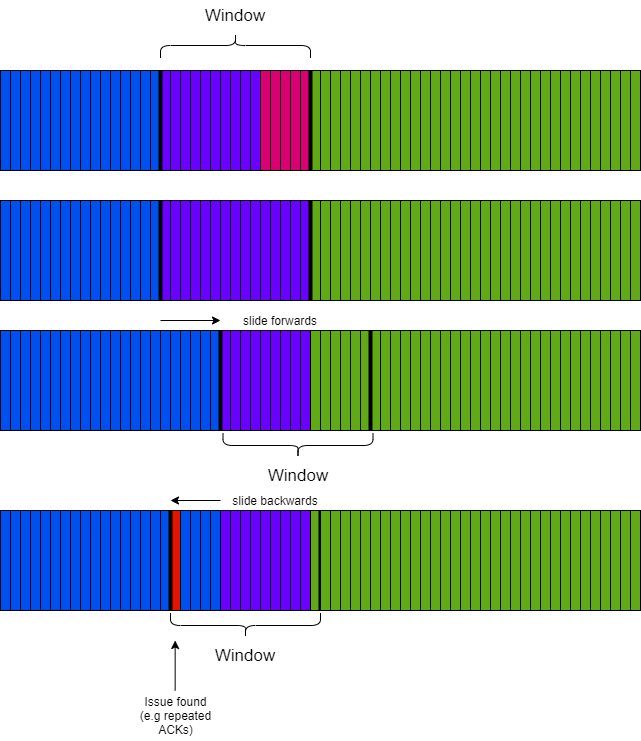
\includegraphics[width=0.7\textwidth]{transport_layer/images/sliding window go back N.png}\end{center}
    Sender transmits multiple segments without waiting for acknowledgement.
    \begin{itemize}
        \setlength\itemsep{0em}
        \item The sender can have up to W bytes of unacknowledged segments in its pipeline.
        \item Sender's state is a queue of acknoledgements.
        \item When we receive some acknoledgements, we can move the slide the window along.
    \end{itemize}
\end{definitionbox}
\begin{definitionbox}{Sliding Window - Selective Repeat}
    Sender only re-transmits those segments it suspects were dropped or corrupted.
    \begin{itemize}
        \setlength\itemsep{0em}
        \item Sender keeps a list/vector of acknowledgements.
        \item Receiver keeps a list/vector of acknowledged segments.
        \item When segments received out of order, they are kept to be added into the data once the missing/gap segments arrive.
        \item Sender keeps a timer for each segment it is waiting for acknowledgement of, resending only when the timer expires.
        \item Sender slides the window when the lowest pending segment is acknowledged.
    \end{itemize}
\end{definitionbox}
\begin{definitionbox}{Flow Control}
    Flow control attempts to prevent the receiver from being overwhelmed/overflowing (rate of sending is too high for it to cope).
    \begin{itemize}
        \setlength\itemsep{0em}
        \item The receiver sends the \textbf{RecieverWindow} size along with acknowledgements.
        \item This typically is the size of buffer left to fill.
        \item When a buffer is full and the receiver can take no more, it sends an acknowledgement with \textbf{RecieverWindow} set to $0$, and repeats a 1-byte ping to the sender to indicate it is not down or deadlocked, but rather just processing.
    \end{itemize}
\end{definitionbox}

\section{Wireless TCP}
\textbf{TCP} was designed before the popularisation of wireless networks.
\\ \begin{minipage}{0.47\textwidth}
    \subsubsection{Wired Network}
    When packets are lost, this indicated congestion.
    \begin{itemize}
        \setlength\itemsep{0em}
        \item Reduce packets sent.
        \item Use congestion avoidance and recovery strategies.
    \end{itemize}
\end{minipage}
\hfill
\begin{minipage}{0.47\textwidth}
    \subsubsection{Wireless Network}
    When packets are lost, this is most likely a channel reliability issue.
    \begin{itemize}
        \setlength\itemsep{0em}
        \item Resend packets as much as possible.
        \item Gives best chance of one getting received correctly.
    \end{itemize}
\end{minipage}
We can fix these conflicting requirements in two ways:
\begin{itemize}
    \setlength\itemsep{0em}
    \bullpara{Split TCP Connections}{
        If we use separate connections for wired and wireless we can distinguish between the two and hence use different algorithms for congestion avoidance.
    }
    \bullpara{Use Base Station}{
        Have the wired base station do some retransmissions without informing the wireless source.
        \\
        \\ Here the base station tries to improve wireless IP reliability using \textbf{TCP}.
    }
\end{itemize}

\section{Network Usage}
\[\text{Utilisation Factor} = \cfrac{\text{network use}}{\text{maximum theoretical usage}}\]
When we have the $RTT$, packet size $L$ and transmission rate $R$, we can also use the time on the connection used out of the possible time length:
\[d_{trans} = \cfrac{L}{R}\]
\[\text{Utilisation Factor} = \cfrac{d_{trans}}{RTT + d_{trans}}\]
